\chapter{Estrutura e Implementação}

Existem já implementadas versões do protocolo \textit{Rollback} Solidário utilizando-se de outras bibliotecas de comunicação e em outras linguagens. A impementação utilizando-se uma biblioteca de agentes móveis implica em algumas características especiais, como a necessidade de haver um servidor de \textit{aglets} em funcionamento em cada estação de trabalho, tal como a intalação da biblioteca de agentes
móveis e da máquina virtual Java.

Como já explicado no capítulo sobre agentes móveis, um agente necessita de um ambiente dedicado para execução. Esse ambiente, neste caso específico para a biblioteca \textit{Aglets} o servidor \textit{Tahiti}, deve estar devidamente instalado e em funcionamento em cada um dos hosts que estarão aptos à fazerem parte do sistema. Cada sessão do ambiente Tahiti está vinculado à um URL e à uma porta (por padrão, o \textit{Tahiti} utiliza a porta 4434). Isso permite a utilização de mais de uma contexto em execução em um mesmo host. A possibilidade de se manter mais de um contexto em execução em uma mesma máquina, para uma aplicação de simulação distribuída, a princípio pode não ser uma vantagem. Mas em tempo de implementação e testes iniciais esta característica foi muito explorada. A implementação deste trabalho foi, por diversos momentos, executados sobre um mesmo ambiente computacional com diversos ambientes Tahiti em execução, um em cada porta, a fim de se simplificar os testes iniciais. Uma vez em estágio mais avançado, os mesmo testes foram aplicados dividindo-se os processos em hosts em pontos distintos de uma rede.

Existem outros pontos que podem ser citados como característica a serem exploradas para o caso da possibilidade de co-existência de diferentes contextos \textit{aglets} em uma mesma máquina, como a possibilidade de manter um processo de execução e o observador em um mesmo ambiente computacional, ou mesmo migrar um processo temporariamente para uma máquina, em caso de manutenção ou interrompimento temporário do funcionamento de um dos \textit{hosts}.

\section{Implementação}

Como todo agente aglet deve ser criado a partir de um ambiente Tahiti, a implementação se inicia por um agente superior, encarregado de criar todos os demais agentes do sistema. Este agente, denominado Servidor, fica encarregado de carregar a lista de hosts do sistema, criar os processos e despachá-los para o seu ambiente de execução. Conforme ilustra o diagrama da Figura~\ref{fig:diagrama_classes} , a implementação conta com seis principais classes:

\begin{itemize}
	\item \textbf{Servidor}: Responsável por iniciar todo o processo. É esta classe que carrega a lista de \textit{hosts} e despacha os processos aos seus hosts de destino;
	\item \textbf{ProcessoPai}: Classe abstrata, que carrega consigo os dados em comum entre um Processo e o Observador;
	\item \textbf{Processo}: Provém toda a estrutura para se tratar um evento. Um processo possui uma lista de eventos a serem tratados. Todo processo tem a capacidade de se comunicar com outro processo qualquer;
	\item \textbf{Evento}: Um evento é uma classe que provém todo o tratamento para execução do código de simulação distribuída;
	\item \textbf{DadosProcesso}: DadosProcesso é a classe que contém os dados referentes a cada  um dos processos em execução, incluso o processo \textit{Observador};
	\item \textbf{Observador}: A classe Observador implementa todo o tratamento de recebimento dos vetores de dependência, eleição de linhas de recuperação, etc.
\end{itemize}

Todo o processo de iniciar os agentes, carregar os dados referentes aos \textit{hosts}, carregar a lista de eventos de cada processo e a inicialização do processo observador é feita no mesmo ambiente onde se executa o processo \textbf{Servidor}. Os processos de execução e o processo observador só iniciam seu funcionamento após chegarem ao seu ambiente de execução (após migração). Isso garante que a criação de um número elevado de agentes não deixe o sistema, em um momento inicial, sobrecarrega, pois o tratamento dos eventos da lista de eventos futuros estará bloqueado enquanto os processos ainda estiverem no mesmo ambiente o qual foram criados (antes de uma migração).

\begin{figure}[htb]
  \centering
  \centerline{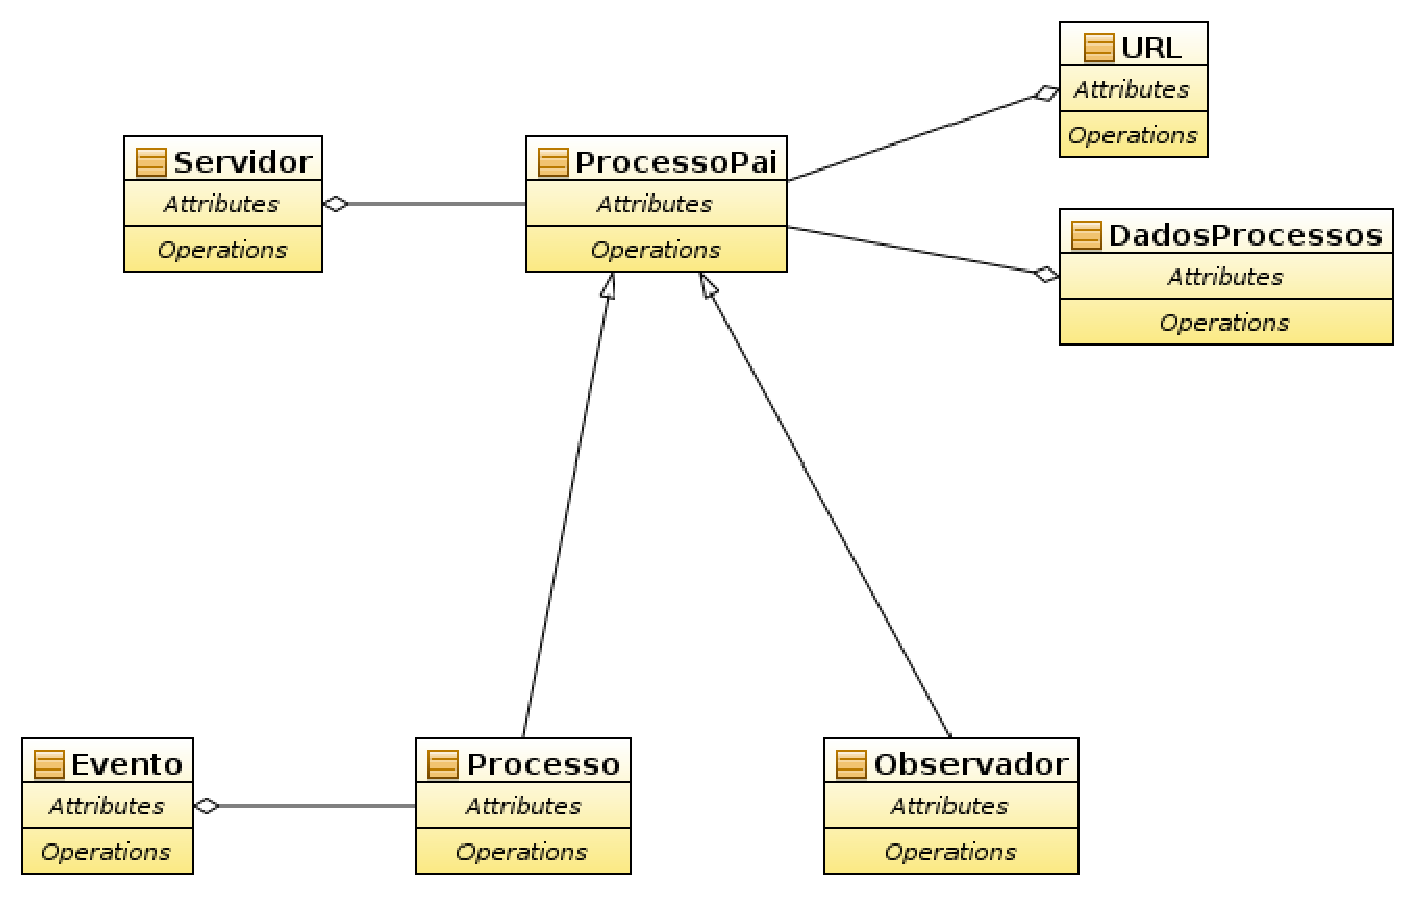
\includegraphics[scale=0.5]{imagens/diagrama_de_classes.eps}}
  \caption{Diagrama de Classes.}
\label{fig:diagrama_classes}
\end{figure}


Cada um dos \textit{hosts} deve estar aptos a receberem um agente \textit{aglet}, com o servidor \textit{Tahiti} devidamente em execução.



\subsection{A Classe Servidor}

A classe Servidor é a responsável por instanciar todos os agentes do sistema. Essa classe deve ser criada já a partir de um servidor \textit{Tahiti}. Ao iniciar, a classe servidor se comporta conforme ilustrado no diagrama da Figura~\ref{fig:diagrama_servidor}. A implementação da classe servidor e seus métodos, conforme ilustrado no diagrama da Figura~\ref{fig:classe_servidor}, são descritos a seguir.



\begin{figure}[htb]
  \centering
  \centerline{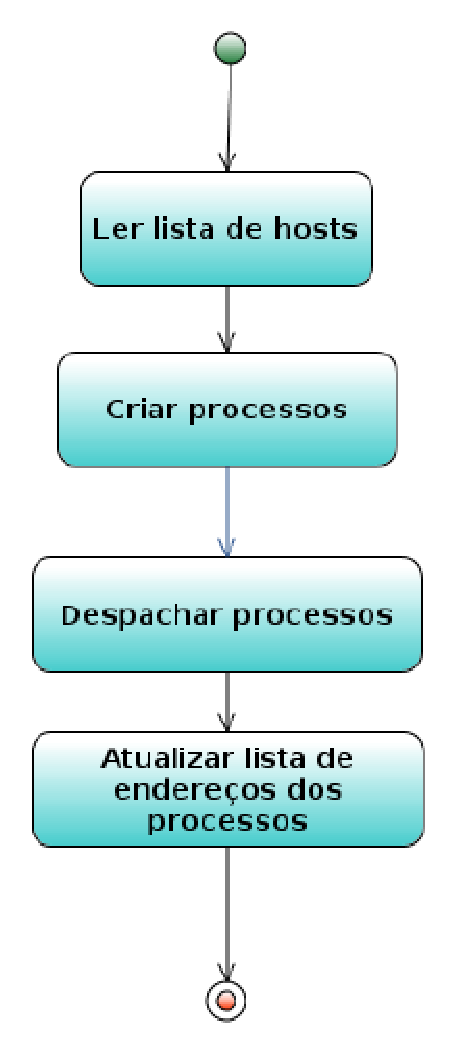
\includegraphics[scale=0.6]{imagens/diagrama_servidor.eps}}
  \caption{ Diagrama de atividades da classe Servidor.}
\label{fig:diagrama_servidor}
\end{figure}

\begin{figure}[htb]
  \centering
  \centerline{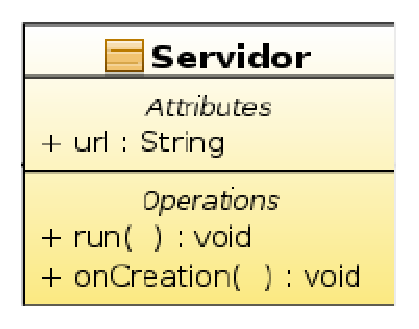
\includegraphics[scale=0.6]{imagens/classe_servidor.eps}}
  \caption{Diagrama da classe Servidor.}
\label{fig:classe_servidor}
\end{figure}


O método \textit{\textbf{onCreationb(Object ini)}}, derivado da classe pai \textit{Aglet}, é executado assim que o agente servidor é instanciado sobre o servidor \textit{Tahiti}. A execução desse método consiste em carregar toda a lista de \textit{Urls} onde serão despachados os processos para serem executados. Ao fim da leitura da lista de hosts, este método se encerra. Como a execução desse método é única em todo o ciclo de vida do agente Servidor, a lista de endereços dos
\textit{Hosts}, assim como a quantidade de processos, não mais será alterada durante a simulação. Em caso de migração de algum processo para um ambiente diferente do ambiente original de simulação, a atualização do novo endereço do processo se dá na lista \textit{DadosProcesso}.

Após a execução do método \textit{\textbf{onCreation(...)}}, o método \textit{\textbf{run()}} assume o controle do agente Servidor. É dentro desse método que os processos são criados (com base na lista de \textit{Urls}. Ao primeiro endereço da lista é atribuído o Processo Observador, os demais endereços são processos de tratamento de eventos. Em um primeiro momento, todos os agentes Processo são criados, e seus dados de controle (\textit{id}, \textit{AgletID} e \textit{LocalProxy}) são armazenados na lista DadosProcessos, para eventuais comunicações. Somente após a criação de todos os processos é que estes agentes são despachados para seus \textit{hosts} de execução. Isso se dá porque cada processo deve conter os dados referentes a todos os processos, inclusive o Observador, para troca de mensagens. Assim que cada agente Processo é enviado para o seu ambiente de execução, os dados relativos aos demais processos são também enviados e, ao chegarem, recompóem a lista \textit{DadosProcesso}.

Ao final do processo de migração de todos os agentes para seus devidos contextos, o agente Servidor encerra sua participação na simulação, e todo o controle a partir desse momento se dá entre os Processos e o Observador.


\subsection{A classe Processo}

A classe Processo é responsável por toda a manipulação dos eventos a serem tratados, tal como a inserção de um novo evento, detecção de mensagem \textit{straggle}, migração, entre outros, conforme pode ser verificado no diagrama da Figura~\ref{fig:diagrama_processo}.

\begin{figure}[htb]
  \centering
  \centerline{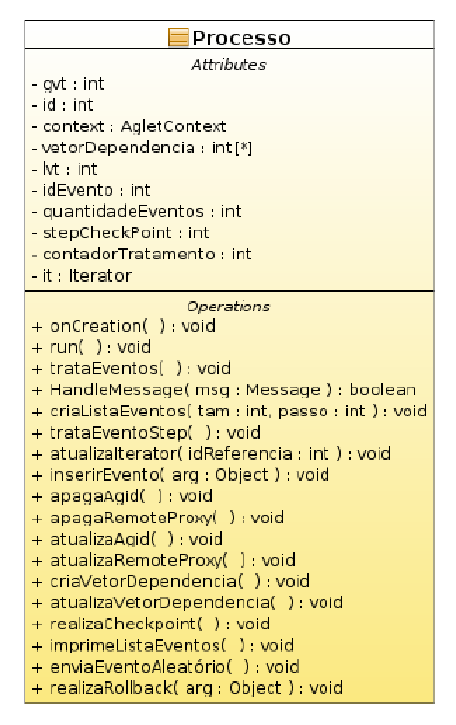
\includegraphics[scale=0.6]{imagens/diagrama_processo.eps}}
  \caption{ Diagrama da classe Processo.}
\label{fig:diagrama_processo}
\end{figure}


Como toda classe derivada da classe \textit{Aglet}, a classe Processo implementa os métodos \textit{\textbf{run()}} e \textit{\textbf{onCreation(...)}}. O método \textit{\textbf{onCreation(...)}} é responsável por criar a lista de eventos futuros e instalar os escutadores (\textit{listeners}) responsáveis pelos eventos de migração e clonagem. Já o método \textit{\textbf{run()}} fica responsável por atualizar o contexto do agente e instanciar o \textit{iterador (iterator)} da lista de eventos futuros. O tratamento dos eventos não é
feito dentro do método \textit{\textbf{run()}} devido ao estilo de migração dos agentes \textit{aglets}. Como a migração de um \textit{aglet} é baseado em mobilidade fraca, caso o tratamento se desse dentro do método \textit{\textbf{run()}} todo o processamento deveria ser refeito caso houvesso uma migração durante a simulação.

A execução do agente processo pode ser dividido em duas partes principais: o tratamento dos eventos da lista de eventos futuro, ilustrado na Figura~\ref{fig:diagrama_tratamento}, e o tratamento do recebimento de mensagens (abordade em uma subcessão específica).

\begin{figure}[htb]
  \centering
  \centerline{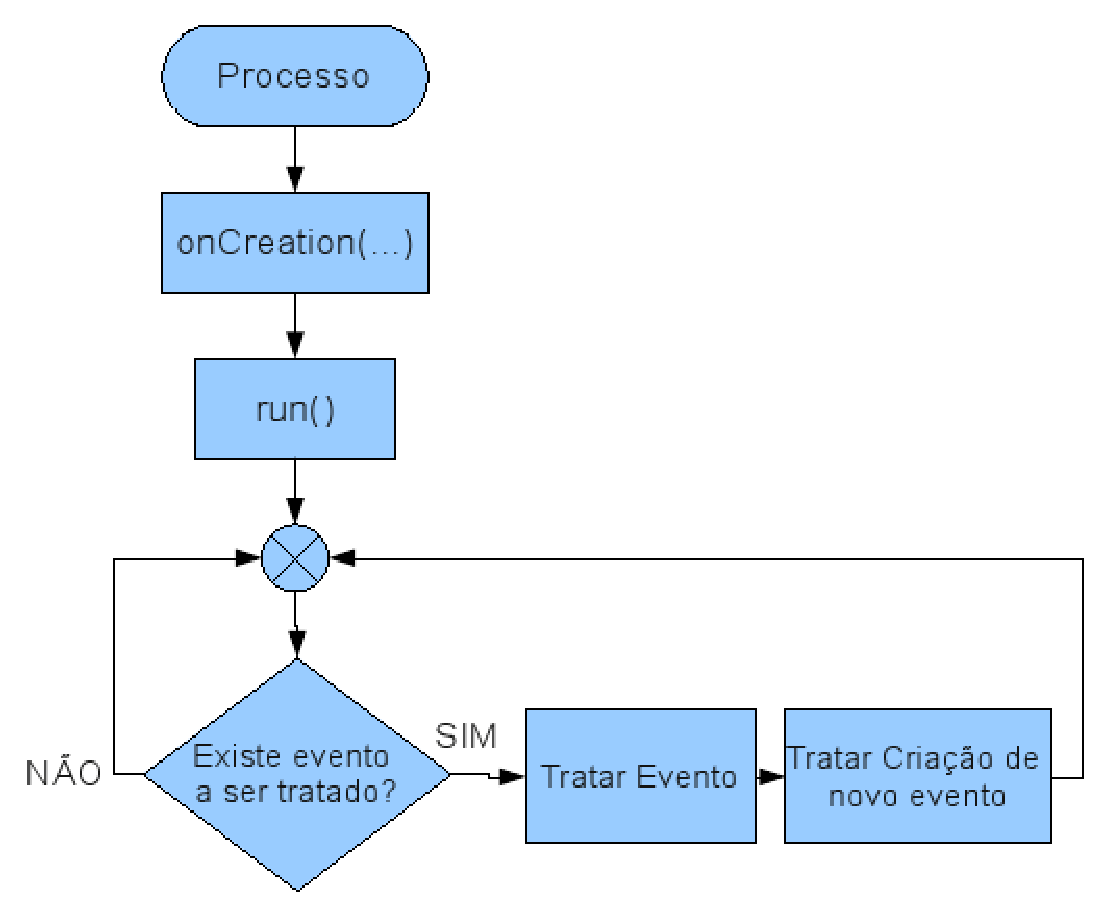
\includegraphics[scale=0.6]{imagens/diagrama_tratamento.eps}}
  \caption{ Tratamendo de eventos na classe Processo.}
\label{fig:diagrama_tratamento}
\end{figure}

O tratamento dos eventos no loop principal do agente \textit{\textbf{Processo}} consiste em retirar o próximo evento da lista de deventos futuros, tratar os dados referentes a esse evento, verificar a criaçào de um novo evento relativo ao processamento atual e retornal ao início do ciclo. Ao finalizar um ciclo de tratamento de eventos, o processo envia uma mensagem para si mesmo, indicando o fim do tratamento de um ciclo. Essa mensagem é colocada na fila de mensagens e é processada pelo método \textit{\textbf{handleMessagem(...)}}, o qual inicia um novo ciclo de tratamento de evento. Esse processo permite a eliminação de um laço do tipo \textit{\textbf{while(...)}} ou um laço \textit{\textbf{for(...)}} para a execução do ciclo de tratamento de eventos. Caso o tratamento se desse dentro de uma das estruturas de repetição citadas, ocorreria um sério problema em relação ao tratamento das mensagens chegas em tempo de execução (essa abordagem será melhor detalhada na subsessão 5.1.4 , sobre tratamento de mensagens).


Existem dois pontos importantes relacionados ao tratamento de eventos: como é feito o tratamento em relação à mobilidade fraca e como é feita a atualização da lista de eventos futuros em caso de recebimento de um novo evento.

Todo o tratamento da lista de eventos futuros é feita com base em uma variável do tipo Iterator. Essa variável é uma interface que permite as operações básicas de percorrer uma coleção. Na implementação do agente Processo, a variável Iterator sempre aponta para o próximo evento a ser tratado.

O método atualizaIterator(...) recebe como parâmetro o LVT do processo atual, e atualiza a variável \textit{Iterator} com base nesse valor. Existem dois principais motivos para a atualização desta variável com base no LVT do processo, os quais garantem o tratamento ininterrupto sobre um agente com mobilidade fraca e a atualização da lista de eventos futuros:

\begin{itemize}
	\item A variável \textit{\textbf{Iterator}} é do tipo não serializável, ou seja, o seu valor não suporta uma migração. Para contornar essa característica, o valor da variável é apagado (recebe \textit{null}) antes da migração e é atualizado com base no LVT ao chegar no seu novo contexto de execução;

	\item Em caso de inserção de um novo evento na lista de eventos futuros, caso esse novo evento seja o vizinho sucessor do atual evento em execução, a variável Iterator apontará para um evento incorreto. Para sanar esse problema, o iterator deve ser atualizado quando essa ocasião acontecer.
\end{itemize}

Existe uma terceira ocasião onde a atualização do \textit{\textbf{Iterator}} é muito importante na simulação: na ocorrência de um \textit{rollback}. Ao ser notificada a realização de um \textit{rollback}, o processo recebe o valor de tempo para o qual deve retornar. Esse valor deve ser utilizado para atualizar o \textit{iterador} da lista de eventos futuros e continuar a simulação.

Existe uma outra gama de métodos implementados que não fazem parte da estrutura do protocolo \textit{Rollback} Solidário, mas que foram inseridas na implementação para dar base de sustentação para testes do funcionamento da implementação. Os métodos \textit{\textbf{criaListaEventos(...)}} e  \textit{\textbf{enviaEventoAleatório(...)}} são, respectivamente, responsáveis por criar uma lista de eventos de um tamanho determinado e enviar um evento aleatório para um processo também aleatório. Esses métodos não fazem sentido para o protocolo em si, mas permitem simular o funcionamento do protocolo em uma ocasião real de simulação.

\subsection{A classe Observador}

	A classe Observador implementa os métodos necessários para o recebimento e tratamento dos checkpoints e para a seleção das linhas de recuperação em caso de rollback. A classe Observador, assim como a classe Processo é derivada da classe ProcessoPai que por sua vez é derivada da classe Aglet. Com isso essa classe carrega as características de um agente aglet e implementa o método run(). São implementados também os demais métodos referentes à inserção de novos vetores de dependência, seleção de linha de recuperação e tratamento de rollback. Os métodos implementados são ilustrados no diagrama da Figura~\cite{fig:classe_observador}.
	

\begin{figure}[htb]
  \centering
  \centerline{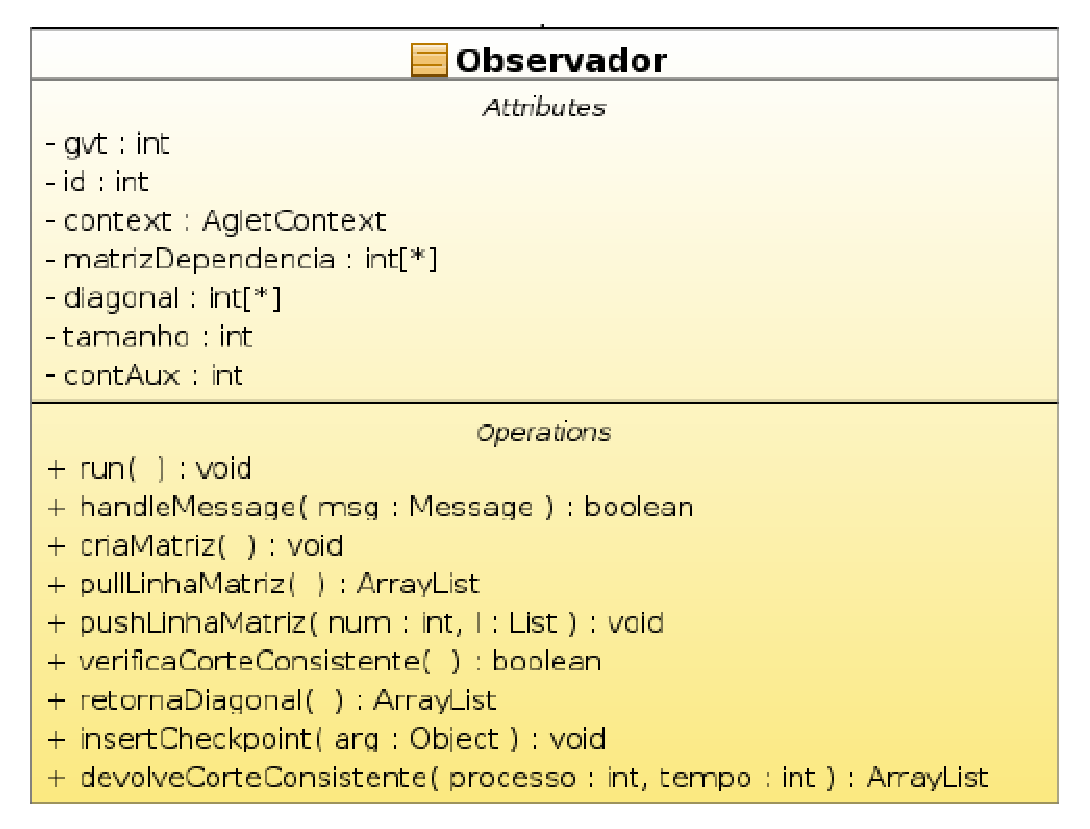
\includegraphics[scale=0.6]{imagens/classe_observador.eps}}
  \caption{Diagrama da classe Observador.}
\label{fig:classe_observador}
\end{figure}
	 
O método \textit{\textbf{run()}} é responsável por atualizar o contexto do agente observador. Após a migração para o seu refrente contexto de execução, o agente observador criar a matriz de dependência, inicializando-a com o valor padrão, ou seja, uma matriz identidade de ordem n onde n é a quantidade de processos em execução. Uma vez criada a matriz, toda a execução é baseada em troca de mensagens. O método  \textit{\textbf{handleMessage(...})} é o responsável por receber e tratar as mensagens. Ao se receber uma mensagem contendo um vetor de dependência (\textit{checkpoint}), o processo Observador verifica se o vetor gera um corte consistente. Caso gere, a linha de recuperação é salva em um vetor de linhas de recuperação. Quando solicitada uma linha de retorno devido ao recebimento de uma mensagem fora da ordem de execução, o método \textit{\textbf{devolveCorteConsistente(...)}} é invocado e retorna a linha de recuperação de menor custo para a simulação.


\subsection{Tratamento de mensagens}

Conforme exposto anteriormente, o tratamento dos eventos dentro da classe \textbf{Processo} não se dá dentro do método \textbf{\textit{run()}}. A razão para isto é não ter que refazer toda a simulação em caso de migração de contexto, devido à mobilidade fraca. A maneira utilizada para se contornar essa situação é fazendo com que um evento inicie o tratamento do próximo evento ao final da sua execução, por meio do envio de uma mensagem \textbf{TrataEvento} (Figura~\cite{fig:trata_evento}). Caso essa abordagem não fosse adotada, todo o tratamento de mensagens seria bloqueado enquanto um processamento (laço \textit{for}/\textit{while}) estivesse em andamento.

\begin{figure}[htb]
  \centering
  \centerline{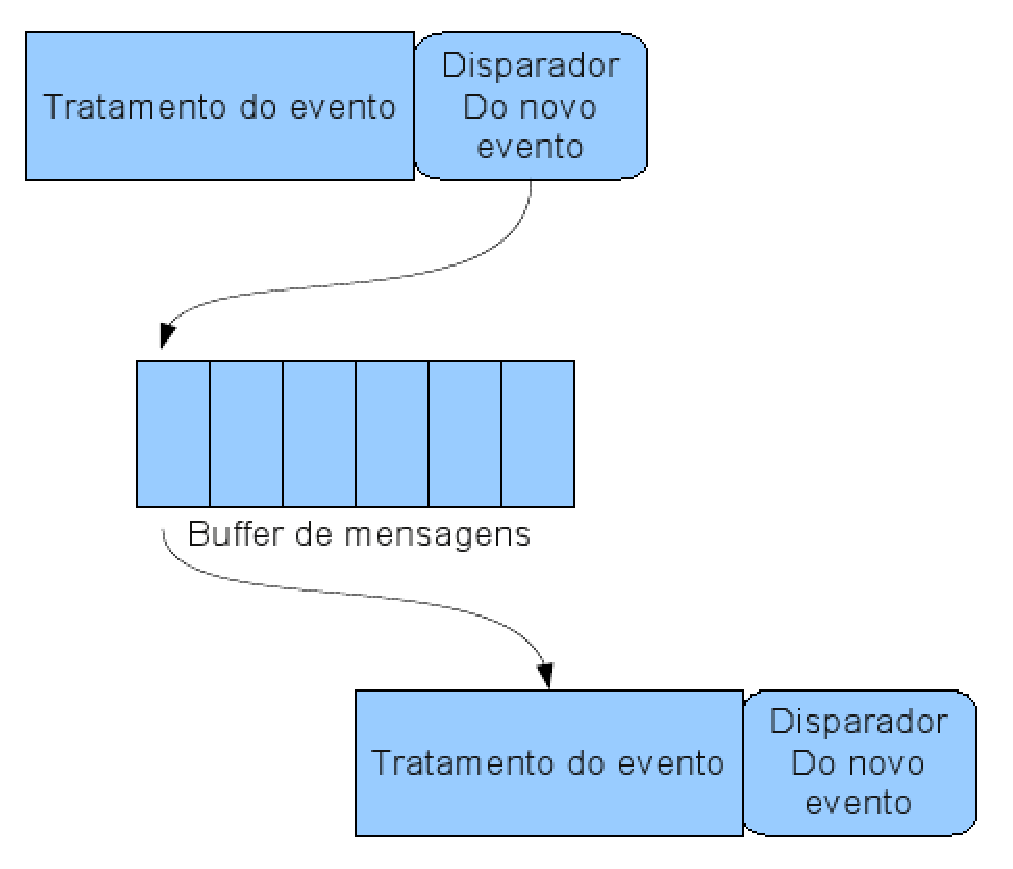
\includegraphics[scale=0.6]{imagens/trata_evento.eps}}
  \caption{ Ciclo de tratamento de eventos.}
\label{fig:trata_evento}
\end{figure}


Ao final do tratamento de um evento, a mensagem é enviada e enfileirada na fila de mensagens para ser tratada pelo processo \textbf{\textit{handleMessage}(...)}. A mensagem em questão recebe o mesmo tratamento que as demais mensagem, e é tratada segundo a ordem em que é recebida. O tratamento das mensagens na ordem em que são recebidas, sem prioridades para algum tipo específico de mensagem, garante a intercalação de execução dos eventos e recebimento de mensagens com eventos externos, mensagens de \textit{rollback} e mensagens de atualização de dados.


Um segundo tipo de mensagem bastante importante no andamento da simulação é a mensagem \textbf{InserirEvento}. Essa mensagem indica a inclusão de um novo evento na lista de eventos futuros do processo, e carrega consigo um objeto do tipo Evento que deve ser alocado na lista de eventos. É com base nos dados desse objeto Evento recebido que se identifica uma mensagem \textit{straggler}, e se dispara otratamento de \textit{rollback}.


Além da mensagem de disparo para tratamento de um novo evento e da mensagem de recebimento de evento existem mensagens referentes à realização de \textit{checkpoint} forçado, migração, realização de \textit{rollback}, inicio do tratamento da lista de eventos, dentre outros. A lista completa de mensagens dos agentes \textbf{Processo} e \textbf{Observador} encontra-se no apêndice ??.

\section{Considerações finais}

	A implementação deste trabalho compreende grande partes das ferramentas necessárias para a implementação de um simulação distribuída utilizando o protocolo \textit{Rollback} Solidário sobre a biblioteca de agentes móveis \textit{Aglets}. Foram desenvolvidas ferramentas para migração, detecção de mensagens recebidas fora da ordem (\textit{straggler}), detecçao de linha de recuperação, em caso de \textit{rollback}, além da estruturação necessária para se inserir um código de simulação distribuída sobre o protocolo.

